%File: AAAI-inst.tex
% support for LaTeX is provided by AAAI, and these instructions
% and the accompanying style files are NOT guaranteed to work.
% If the results you obtain are not in accordance with the 
% specifications you received in your packet (or online), you
% must correct the style files or macro to achieve the correct
% result. 
%

%
% The instructions herein are provided as a general guide for 
% experienced LaTeX users who would like to use that software
% to format their paper for an AAAI Press proceedings or technical
% report or AAAI working notes. These instructions are generic. 
% Consequently, they do not include specific dates, page charges, and so forth. 
% Please consult your specific written conference instructions for 
% details regarding your submission.
%
% Acknowledgments
% The preparation of the \LaTeX{} and Bib\TeX{} files that
% implement these instructions was supported by 
% Schlumberger Palo Alto Research, AT\&T Bell
% Laboratories, Morgan Kaufmann Publishers, and AAAI Press.
\documentclass[letterpaper]{article}
\usepackage{aaai}
\usepackage{times}
\usepackage{helvet}
\usepackage{courier}
\usepackage{amsfonts}
\usepackage{amsmath}
\usepackage{graphicx}

\begin{document}
% The file aaai.sty is the style file for AAAI Press 
% proceedings, working notes, and technical reports.
%
%\title{Model Selection for Causal Inference using Deep Neural Networks}
% TODO: What about 
%\title{Architecture Learning for Deep Counterfactual Networks}
\title{Architecture Learning of Deep Neural Networks for Counterfactual Inference}
\author{Author One, Author Two, Author Three\\
Authors Details\\
Authors Email}
\maketitle


\begin{abstract}
\begin{quote}
We propose a novel approach for automatically inferring appropriate architectures of deep neural networks for the task of counterfactual inference over observational data. The individualised causal effect of an intervention or treatment is modelled in terms of  a multi-task learning  problem using a deep neural network which consists of a number of layers that are shared among the factual and counterfactual outcomes and a number of outcome-specific layers. Our approach enables automatically selecting an appropriate architecture (i.e. number of shared and outcome-specific layers) by exploiting inferred characteristics of the dataset such as the propensity score, the skewness of the data, and the complexity of the different outcome functions.
We conduct experiments on a synthetic dataset allowing us to parametrize and fully control the characteristics of the data before applying our approach to a real-world observational study for which we infer the characteristics in order to derive an appropriate architecture. As shown in the experiments, our method outperforms the state-of-the-art.
 
\end{quote}
\end{abstract}


\section{Introduction}
The technological advancements of recent years have resulted in an increasing availability of data in various fields such as healthcare, education, and economics. This data can be used to make predictions concerning unseen data points on the basis of statistical models. When dealing with observational studies, we are often particularly interested in the task of predicting the individualised treatment effect that certain intervention has on a given subject or context. In the case of electronic health records, for instance, a dataset typically consists of a set of patients each with individual features, a treatment assignment indicator (i.e. whether or not they received the treatment), and an observed outcome which we call the \emph{factual outcome}. The quantity we are interested in is the \emph{counterfactual outcome} (i.e. the outcome had the patient received a different treatment assignment) because it allows us to compute the individualised treatment effect helping us make informed decision during treatment planning. % TODO Add sources


% TODO Check how much I can take from Ahmed's Sentence
% TODO Prove-read. It's full of spelling mistakes
Classical works have focused on estimating “aver- age” treatment effects through variants of propensity score matching (Rubin, 2011; Austin, 2011; Abadie  Imbens, 2016; Rosenbaum  Rubin, 1983; Rubin, 1973). More recent works tackled the problem of estimating “indi- vidualized” treatment effects using representation learn- ing (Johansson et al., 2016; Shalit et al., 2017), Bayesian inference (Hill, 2012), and standard supervised learning (Wager  Athey, 2015). \\

% TODO Cite our own paper
Recent works have shown that the problem can be effectively framed in terms of a multi-task learning problem using deep neural networks. The network has a set of layers that are shared among both the factual and the counterfactual outcomes and a number of outcome-specific layers. However, the questions of how to select an appropriate architecture (i.e. the number of shared layers, and the number of outcome-specific layers) may drastically influence the expressiveness and computational complexity of the model and remains an open challenge. While there are various general approaches for model selection and architecture learning in neural networks, they do not make use of the specific nature of our causal inference problem. % TODO Quote Model selection papers
 \\

In this paper, we propose a novel approach for automatically inferring appropriate architectures of deep neural networks for the task of counterfactual inference over observational data. This is achieved by exploiting inferred characteristics of the dataset such as the propensity score, the skewness of the data, and the complexity of the different outcome functions. For instance, if one of the outcomes follows a much more complex function than the other, this should be reflected in an asymmetric architecture which utilises a higher number of outcome-specific layers for the more complex outcome than for the other. 


%This is my introduction
%* What is counterfactual inference
%* Why does it matter?
%* Application areas
%
%* What is deep learning? 
%* Why is it appropriate for causal inference
%* We use multi-task learning
%
%* Which datasets? 
%
%* Model selection for deep learning is difficult
%* There are various methods, but they don't exploit the specific nature of causal inference
% TODO: Do I need a dedicated Related Works Section or is implicit in the introduction? 
%\section{Related Works}
%% TODO Check related works
%* Deep Learning
%* Model selection (Optimal Brain Damage, Optimal Brain Surgeon) 
%* Causal Inference using Deep Neural Nets (Sontag et al)
%* Our other ICML paper


\section{Problem Formulation}
% TODO Check if it's okay that this is so similiar to previous paper
% TODO cite Rubin 2011
We represent each subject $i$ in our population  with a $d$-dimensional feature vector $X_i \in \mathcal{X}$, and two \emph{potential outcomes} $Y_{i}^{(1)}, Y_{i}^{(0)} \in \mathbb{R}$ which are drawn from a distribution $(Y_{i}^{(1)}, Y_{i}^{(0)}) \mid X_i = x \sim \mathbb{P}(\cdot \mid X_i = x)$. This way, the \emph{individualised treatment effect} for subject $i$ can be expressed as 

\[
T(x) = \mathbb{E}[Y_{i}^{(1)} - Y_{i}^{(0)} \mid X_i = x] . \tag{1} \label{eq:ite}
\]

Given this definition, the objective is to approximate the function $T(x)$ using an observational dataset $\mathcal{D}$ consisting of $n$ independent samples. Each sample is comprised of a tuple $ \langle X_i, W_i, Y_{i}^{(W_i)} \rangle$, where $X_i$ represents the subject's features, $W_i \in \{0,1\}$ the treatment assignment indicator, and $Y_{i}^{(W_i)}$ and $Y_{i}^{(1 - W_i)}$ the respective \emph{factual} and \emph{counterfactual} outcome. 
The treatment assignment is a random variable depending on the subjects' features, i.e. $W_i \not \perp X_i$. The assignment reflects a domain-specific policy which can be captured in terms of the probability $p(x) = \mathbb{P}(W_i = 1 \mid X_i = x)$ which is called the \emph{propensity score}. \\

% TODO Quote Rubin
% TODO Describe multi-task learning
% TODO What is the formalism of what we want to show here? 
%
%* What does Model Selection mean? 
%* Which objective function are we trying to optimise
We are following the approach of (TODO CITATION)
% TODO CITE our own paper
and are using a \emph{deep counterfactual network} (DCN) to infer $T(x)$ from $\mathcal{D}$. The DCN treats the problem as a multi-task learning problem using a deep neural network with an architecture illustrated in figure \ref{fig:dcn-architecture}. 
The network uses a number $L_s$ of shared layers, a number $L_{i,0}$ of idiosyncratic layers for the \emph{treated outcome}, and a number $L_{i,1}$ for the \emph{control outcome}. We are interested in learning an appropriate architecture of the DCN, in particular, coming up with suitable values for $L_s$, $L_{i,0}$, and $L_{i,1}$. 


\begin{figure}
	\centering
	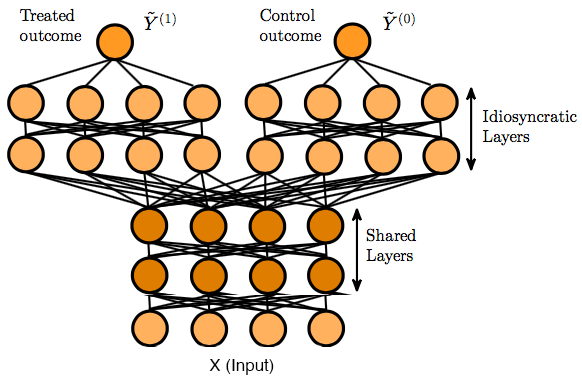
\includegraphics[width=0.5\textwidth]{img/fig-dcn-architecture.png}
	\caption{DRAFT: Architecture of a Deep Counterfactual Network (DCN). Objective is to learn appropriate values for number the different number of layers (here $L_s = L_{i,0} = L_{i,1} = 2$).}
\end{figure}

\section{Architecture Learning}
* How does architecture learning work in general? \\
* What are the main existing methods for this? \\

* What is our approach? \\
* Hyper-parameter search that is informed by propensity score and different metrics of the data \\

\subsection{Relevant Characteristics}
Briefly describe ...

\subsubsection{(a) Skewness}
* What do we mean by that?  \\% TODO Or should that go to the formalism section? 
* Depending on propensity score. \\
* How do we get that the PS? \\
* How should it be reflected in the layers? \\
* How does it influence the architecture? \\
* Qualitatively? Quantitatively? \\
* out1 / total, out2 / total \\

\subsubsection{(b) Complexity of Response Surfaces}
* What do we mean by that? \\ % TODO Or should that go to the formalism section? 
* What does it depend on? \\ 
* How do we measure it? \\
* How should it be reflected in the layers? \\
* How does it influence the architecture? \\
* Qualitatively? Quantitatively? \\
* shared / total or out1 / total, out2 / total ? \\

\subsubsection{(c) Interdependence between Features}
* What do we mean by that? \\ % TODO Or should that go to the formalism section? 
* What does it depend on?  \\
* How do we measure it? \\
* How should it be reflected in the layers? \\
* How does it influence the architecture? \\
* Qualitatively? Quantitatively? \\
* shared / total\\

\subsection{Deriving a suitable Architecture for the DCN} 
* Once we are able to quantify these characteristics, what do we do with it? \\ 
* What is the relationship between these characteristics and an appropriate architecture? 

% TODO: Do we need to train the model (e.g. using characteristics-based objective function). If so, this would be the section:
%\subsection{Training the Model}
%* How does the training algorithm work?
%* How do we compute the quantities / characteristics / statistics? 
%* Show pseudocode of algorithm





\section{Experiments}
The experiments are conducted on two different datasets. Firstly, we use a synthetic model which allows us to parametrise and fully control the characteristics mentioned in the previous section. This gives us the power to investigate how the different characteristics influence the performance of the learnt architecture.
Secondly, we run the experiments on the \emph{UNOS} dataset % TODO Cite UNOS
(consisting of information regarding patients who went an organ transplantation) to show how our approach generalises to a real-world dataset for which we do not have access to the characteristics directly. Therefore, we are inferring them from the data in order to learn a suitable architecture. 
In both cases, we compare the performance of a DCN whose architecture was learnt by our approach to a generic DCN and a number of other baseline approaches and architectures.  \\

As we are dealing with counterfactual inference, we generally 




* Problem of counterfactual inference
* How do we evaluate performance

* In order to show that it our approach generalises and works on real-world dataset, we use UNOS dataset \\
* Neither control nor knowledge over the characteristics \\
* We need to infer them / learn them as described above
* We compare a variety of different models (incl default DCN, and DCN with inferred architecture) \\

* How were the experiments conducted? 
* Implemented in Tensorflow 


\subsection{Synthetic Model}
\subsubsection{Data Generation}
* Synthetic model \\
* Want to have control over all parameters \\
* Skewness, Propensity Score, General Complexity, Complexity for different outcomes \\
* How did we generate it \\

\subsubsection{Results and Discussion}
* Describe settings: Number of samples, experiments, hyper-params, etc. \\
* Show result table

\subsection{UNOS Dataset}
Real-world dataset to illustrate how our approach generalises

\subsubsection{About the dataset}
* Who is the provider? \\
* What is it about? \\
* Some statistics: Samples, Features, etc. \\
* What is the treatment assignment, what the outcome? \\

\subsubsection{Results and Discussion}
* Describe settings: Number of samples, experiments, hyper-params, etc. \\
* Show result table
* Details of experiment
* Show graph
* Explore the different parameters
* Synthetic Model and Mapping it to real dataset


\section{Conclusions and Future Research}
Counterfactual inference over observational data is of great importance in various areas such as healthcare, education, and economics. Deep neural networks are highly suitable for the task and represent the state-of-the art as they are able to capture complex relations in the outcome surfaces. However, it remains and open challenge of how to select an appropriate architecture for models. This is true in particular in the case of \emph{deep counterfactual networks} which treat the problem as a multi-task learning problem with different numbers of shared and outcome-specific layers.

Our approach addresses this issue of model selection and provides an effective way to automatically learn a suitable architecture by inferring relevant characteristics from the data and incorporating them into the model selection. As shown in the experiments, our approach outperforms the state-of-the-art. 

% TODO Include future work
% * Extend to non-binary case. 
% * Might be particularily relevant because the architectural choice are even bigger. More paremeters to explore. 

%\section{Future Work}
%Future Work
%* Extend this to time-series
%* Extend to non-binary case
% TODO Think of more future work


% TODO Remove pagebreak
\pagebreak
\bibliography{sources}{}

\bibliographystyle{apalike}




% TODO Should I add acknowledgments
%\section{Acknowledgments}
%Acknowledgements


\end{document}
